% The architecture figure in fleetwatch-overview.tex, drawn in TikZ.
% Build with: tectonic docs/figures/architecture.tex   (writes architecture.pdf beside it)
\documentclass[tikz, border=4pt]{standalone}
\usepackage{fontspec}
\setmainfont{texgyreheros}[Extension=.otf, UprightFont=*-regular,
  BoldFont=*-bold, ItalicFont=*-italic, BoldItalicFont=*-bolditalic]
\setmonofont{texgyrecursor}[Extension=.otf, UprightFont=*-regular,
  BoldFont=*-bold, ItalicFont=*-italic, BoldItalicFont=*-bolditalic]
\usetikzlibrary{positioning, arrows.meta, calc}

% The logo's colours: navy ground, teal sweep, amber blip.
\definecolor{navy}{HTML}{1F2E4A}
\definecolor{teal}{HTML}{3E8E7E}
\definecolor{tealbg}{HTML}{E3F3EE}
\definecolor{amber}{HTML}{C98A1A}
\definecolor{amberbg}{HTML}{FBF0DA}
\definecolor{greybg}{HTML}{F1F2F4}

\begin{document}
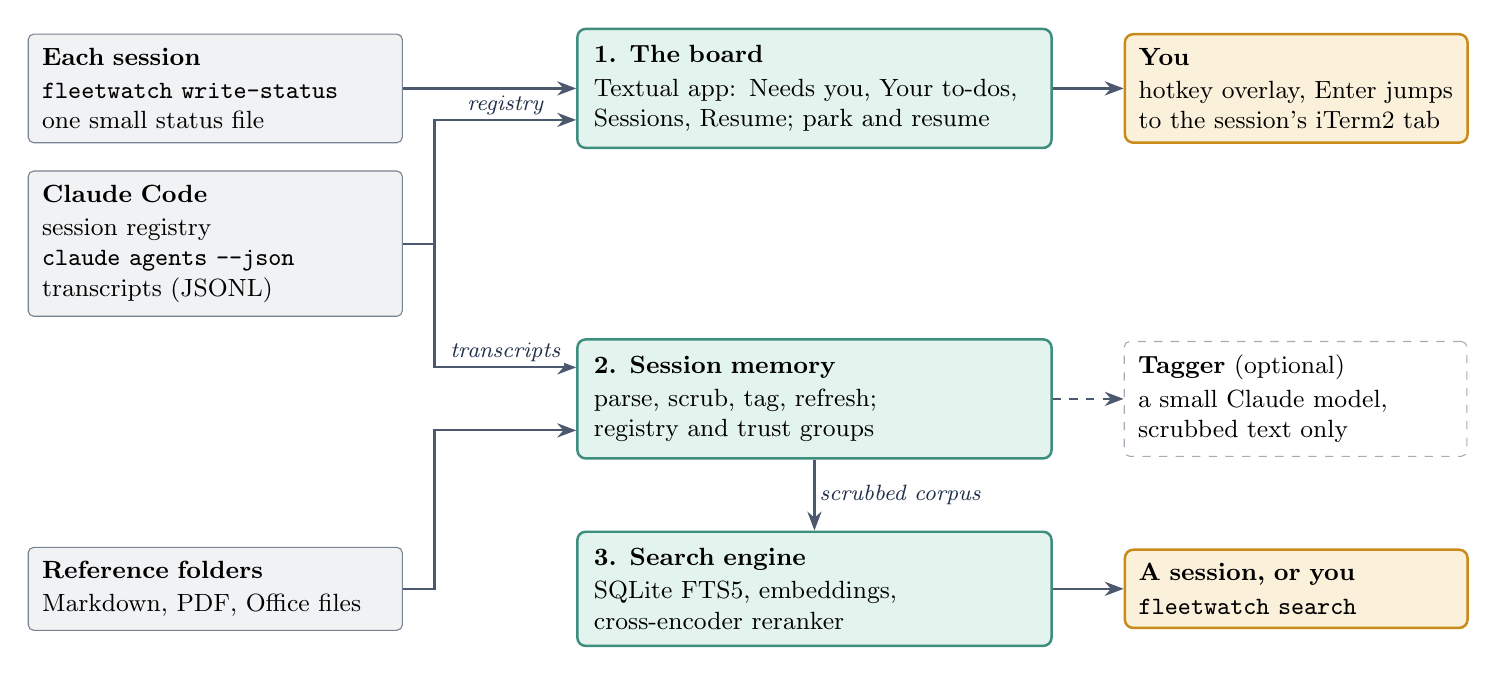
\begin{tikzpicture}[
    font=\small,
    node distance=7mm and 9mm,
    src/.style={draw=navy!60, fill=greybg, rounded corners=2pt, align=left,
      inner sep=5pt, text width=44mm},
    layer/.style={draw=teal, line width=0.9pt, fill=tealbg, rounded corners=3pt,
      align=left, inner sep=6pt, text width=56mm},
    dest/.style={draw=amber, line width=0.9pt, fill=amberbg, rounded corners=3pt,
      align=left, inner sep=5pt, text width=40mm},
    flow/.style={-{Stealth[length=2.4mm]}, line width=0.8pt, draw=navy!80},
    lab/.style={font=\footnotesize\itshape, fill=white, inner sep=1.5pt, text=navy},
  ]

  % The three layers, middle column
  \node[layer] (board) {\textbf{1. The board}\\[1pt]
    Textual app: Needs you, Your to-dos,\\ Sessions, Resume; park and resume};
  \node[layer, below=24mm of board] (memory) {\textbf{2. Session memory}\\[1pt]
    parse, scrub, tag, refresh;\\ registry and trust groups};
  \node[layer, below=9mm of memory] (engine) {\textbf{3. Search engine}\\[1pt]
    SQLite FTS5, embeddings,\\ cross-encoder reranker};

  % Inputs, left column
  \node[src, left=22mm of board] (status) {\textbf{Each session}\\[1pt]
    \texttt{fleetwatch write-status}\\ one small status file};
  \node[src, left=22mm of $(board.south west)!0.5!(memory.north west)$] (claude)
    {\textbf{Claude Code}\\[1pt] session registry\\ \texttt{claude agents -{}-json}\\ transcripts (JSONL)};
  \node[src, left=22mm of engine] (docs) {\textbf{Reference folders}\\[1pt]
    Markdown, PDF, Office files};

  % Outputs, right column
  \node[dest, right=of board] (you) {\textbf{You}\\[1pt]
    hotkey overlay, Enter jumps\\ to the session's iTerm2 tab};
  \node[draw=navy!40, dashed, rounded corners=2pt, align=left, inner sep=5pt,
    text width=40mm, right=of memory] (tagger) {\textbf{Tagger} (optional)\\[1pt]
    a small Claude model,\\ scrubbed text only};
  \node[dest, right=of engine] (search) {\textbf{A session, or you}\\[1pt]
    \texttt{fleetwatch search}};

  % Flows. Claude Code's two arrows share one vertical channel; they cover
  % different heights, so they never overlap.
  \draw[flow] (status.east) -- (board.west |- status.east);
  \draw[flow] (claude.east) -- ++(4mm,0) |- node[lab, pos=0.75, above] {registry} ([yshift=-4mm]board.west);
  \draw[flow] (claude.east) -- ++(4mm,0) |- node[lab, pos=0.75, above] {transcripts} ([yshift=4mm]memory.west);
  \draw[flow] (docs.east) -- ++(4mm,0) |- ([yshift=-4mm]memory.west);
  \draw[flow] (memory.south) -- node[lab, right] {scrubbed corpus} (engine.north);
  \draw[flow] (board.east) -- (you.west);
  \draw[flow, dashed] (memory.east) -- (tagger.west);
  \draw[flow] (engine.east) -- (search.west);
\end{tikzpicture}
\end{document}
